We choose to implement an Image Style Transfer system.
Providing two images, one being aimed to give the content and the other the style, the product tries to be artistic or even amusing.\\
The theoretical basis for this work is given by \emph{"A Neural Algorithm of Artistic Style", Gatis, Ecker \& Bethge (2015)}\footnote{\href{https://arxiv.org/abs/1508.06576}{https://arxiv.org/abs/1508.06576}},
and our code is strongly influenced by the Keras library example on Neural Style Transfer\footnote{\href{https://keras.io/examples/generative/neural\_style\_transfer/}{https://keras.io/examples/generative/neural\_style\_transfer/}}.

\subsection{Explanation}
The implemented system uses a Convolutional Neural Network (CNN), optimizing three different loss functions, to separate and recombine the content of one arbitrary image and the style of another.\\
\subsubsection{Content Loss}
While passing an image through a CNN, its representations become increasingly careful about its content,
leaving aside the details about the actual value of each pixel, especially in higher layers of the network.\\
Being specific, the content loss is a L2 (Euclidean) distance between the features of the base image (extracted from a deep layer of the CNN) and the features of the new image, keeping the generated image close enough to the original one.

\subsubsection{Gram Matrix}
Given a set $V$ of m vectors (points in $R^n$), the Gram matrix $G$ is the matrix of all possible inner products of $V$, i.e.,
\begin{center}
    \(
     g_(ij)=v_i^Tv_j 
    \)
\end{center}
where \(A^T\) denotes the transpose.
The Gram matrix determines the vectors $v_i$ up to isometry
\footnote{Weisstein, Eric W. "Gram Matrix." From MathWorld--A Wolfram Web Resource. \href{https://mathworld.wolfram.com/GramMatrix.html}{https://mathworld.wolfram.com/GramMatrix.html}}.

\subsection{Implementation}
From a most abstract level, our implementation consists of:
\begin{itemize}
    \item Choosing images and weights for content and style
    \item Setting up the network (includes applying Transfer Learning from a VGG-19 network)
    \item Preprocessing the content and style images
    \item Training the network: at this point (for any number of iterations), we may extract the combination image from the network
    \item Printing the result
\end{itemize}
\subsubsection{Content and Style images}
For our experiment, we decide to use free-licensed images from Imgur\footnote{\href{https://imgur.com/}{https://imgur.com/}}.
As a default (proven that it gives good results), we define the content weight to be lower than the style weight and the total variation weight:
\begin{itemize}
    \item $total_variation_weight = 0.000001$
    \item $style_weight = 0.000001$
    \item $content_weight = 0.000000025$
\end{itemize}
\subsubsection{VGG-19}
VGG\footnote{\href{https://arxiv.org/abs/1409.1556}{\emph{"Very Deep Convolutional Networks for Large-Scale Image Recognition", Simonyan \& Zisserman (2015):} https://arxiv.org/abs/1409.1556}}
is a CNN near human performance on common visual object recognition tasks.
There are several representations of it, named after the number of convolutional layers (such as VGG-16 and VGG-19).
For this project, the selected one is \emph{VGG-19}, pre-trained on \emph{ImageNet} and provided by the Keras library
\footnote{\href{https://keras.io/api/applications/vgg/}{https://keras.io/api/applications/vgg/}}. It consists of the following layers:
\begin{multicols}{2}
    \begin{enumerate}
        \item Conv3x3 (64 filters)
        \item Conv3x3 (64)\\
        MaxPool
        \item Conv3x3 (128)
        \item Conv3x3 (128)\\
        MaxPool
        \item Conv3x3 (256)
        \item Conv3x3 (256)
        \item Conv3x3 (256)
        \item Conv3x3 (256)\\
        MaxPool
        \item Conv3x3 (512)
        \item Conv3x3 (512)
        \item Conv3x3 (512)
        \item Conv3x3 (512)\\
        MaxPool
        \item Conv3x3 (512)
        \item Conv3x3 (512)
        \item Conv3x3 (512)
        \item Conv3x3 (512)\\
        MaxPool
        \item Fully Connected (4096 neurons)
        \item Fully Connected (4096)
        \item Fully Connected (1000)\\\\
        SoftMax
    \end{enumerate}
\end{multicols}
Since we care exclusively about the representations of the image, and not about condensing them into any kind of prediction,
we leave aside the Dense (Fully Connected) layers.
\subsubsection{Setup}
Other than providing custom names to layers, we need a model to extract the features at intermediate stages of the training (we actually never get to the end), so we do that.\\
Also, we need to define the optimizer to use during the training: we select a simple Stochastic Gradient Descent\footnote{\href{https://towardsdatascience.com/stochastic-gradient-descent-clearly-explained-53d239905d31}{https://towardsdatascience.com/stochastic-gradient-descent-clearly-explained-53d239905d31}},
setting an Exponential Decay\footnote{\href{https://en.wikipedia.org/wiki/Exponential\_decay}{https://en.wikipedia.org/wiki/Exponential\_decay}},
in order to begin reducing the losses rapidly, and reduce that velocity once we are refining details.
The actual used values are the following:
\begin{itemize}
    \item initial learning rate = 100.0
    \item decay steps = 100,
    \item decay rate = 0.96
\end{itemize}
\subsubsection{Fine Tuning}
For this particular problem, fine tuning is not aiming to improve the accuracy (or any other score) of the model,
but just providing a tool to generate better artistic results, maybe reducing the time to achieve so.\\
In the next subsection (\emph{Examples}), we show some of these different variations. For example:
\begin{itemize}
    \item For the chosen images (the scuba diver for content, the mosaics for style), giving less weight to content makes a decent result at just 500 iterations, showing almost no difference at 4000.
    \item Updating the content weight to be higher (0.00001), the person and the fish on the picture are more identifiable while maintaining the mosaic style (again, 500 and 4000 iterations give similar results).
    \item For a second pair of images (a spider for content, an abstract-ish watercolor bouquet of flowers for style), setting a higher content weight prevents the combination to fully capture the style.
\end{itemize}

\clearpage
\subsection{Examples}
\begin{multicols}{2}
    \begin{center}
        \captionsetup{type=figure}
        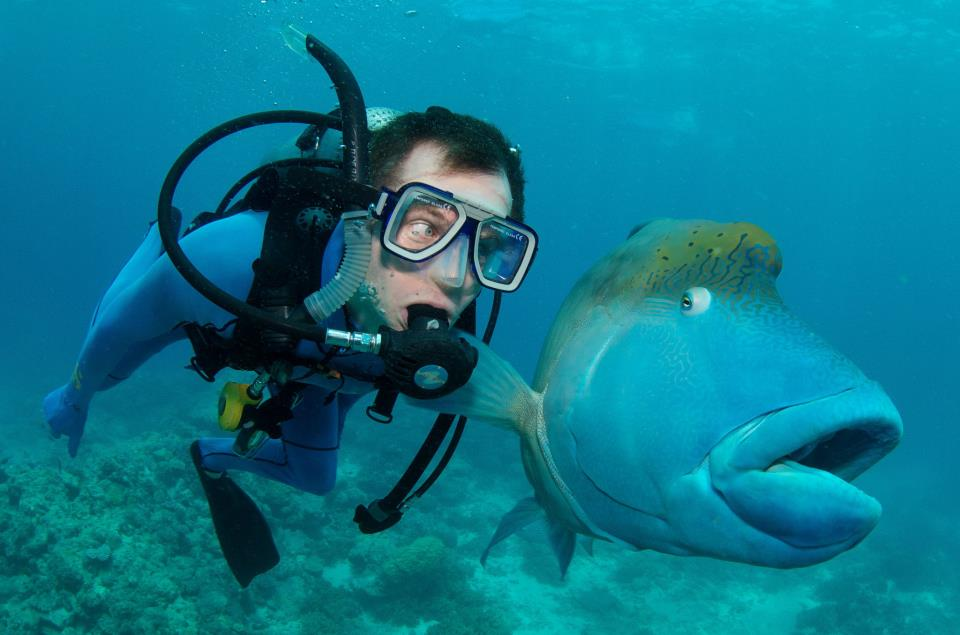
\includegraphics[width=200px, height=200px]{images/dive.jpeg}
        \captionof{figure}{Scuba Diver}\footnote{\href{https://i.imgur.com/B06clk7.jpeg}{https://i.imgur.com/B06clk7.jpeg}}
    \end{center}
    \begin{center}
        \captionsetup{type=figure}
        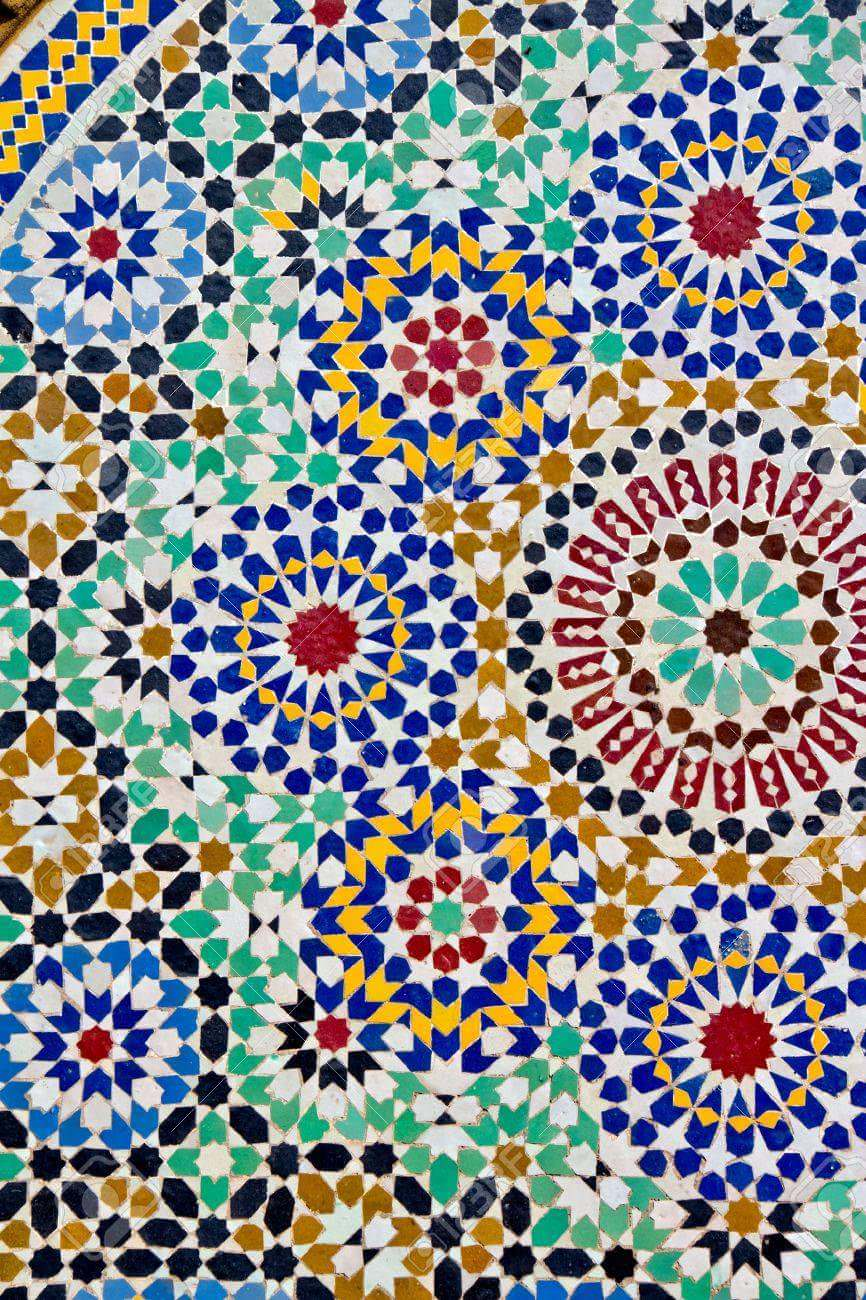
\includegraphics[width=200px, height=200px]{images/mosaic.jpeg}
        \captionof{figure}{Mosaics}\footnote{\href{https://i.imgur.com/F7t3pzM.jpeg}{https://i.imgur.com/F7t3pzM.jpeg}}
    \end{center}
\end{multicols}
\begin{multicols}{2}
    \begin{center}
        \captionsetup{type=figure}
        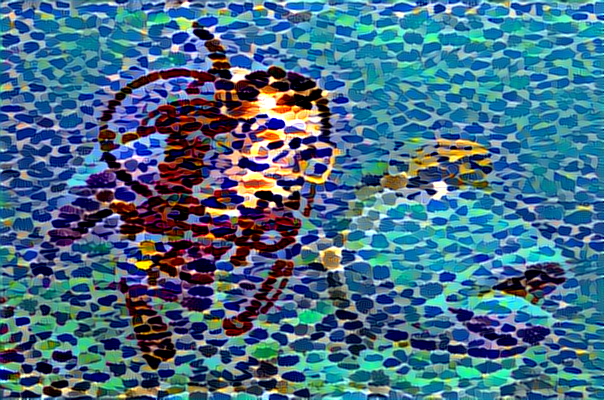
\includegraphics[width=200px, height=200px]{images/comb-mosaic-2.png}
        \captionof{figure}{Mosaic Scuba Diver (content=0.000000025 style=0.000001)}
    \end{center}
    \begin{center}
        \captionsetup{type=figure}
        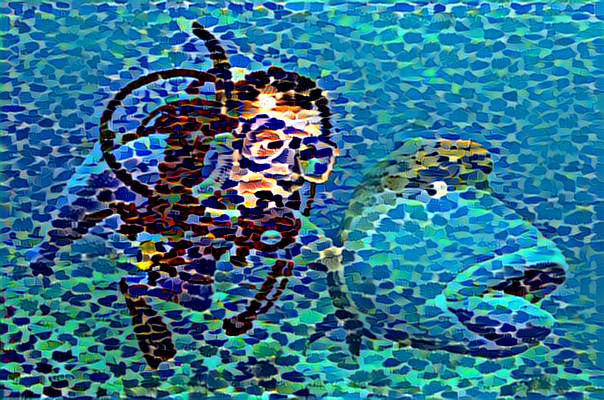
\includegraphics[width=200px, height=200px]{images/comb-mosaic-3.png}
        \captionof{figure}{Mosaic Scuba Diver (content=0.00001 style=0.000001)}
    \end{center}
\end{multicols}
\begin{multicols}{2}
    \begin{center}
        \captionsetup{type=figure}
        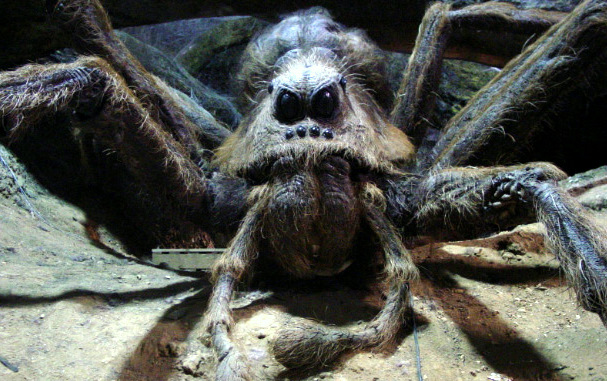
\includegraphics[width=200px, height=200px]{images/aragog.jpeg}
        \captionof{figure}{Big Spider}\footnote{\href{https://i.imgur.com/695mU3B.jpeg}{https://i.imgur.com/695mU3B.jpeg}}
    \end{center}
    \begin{center}
        \captionsetup{type=figure}
        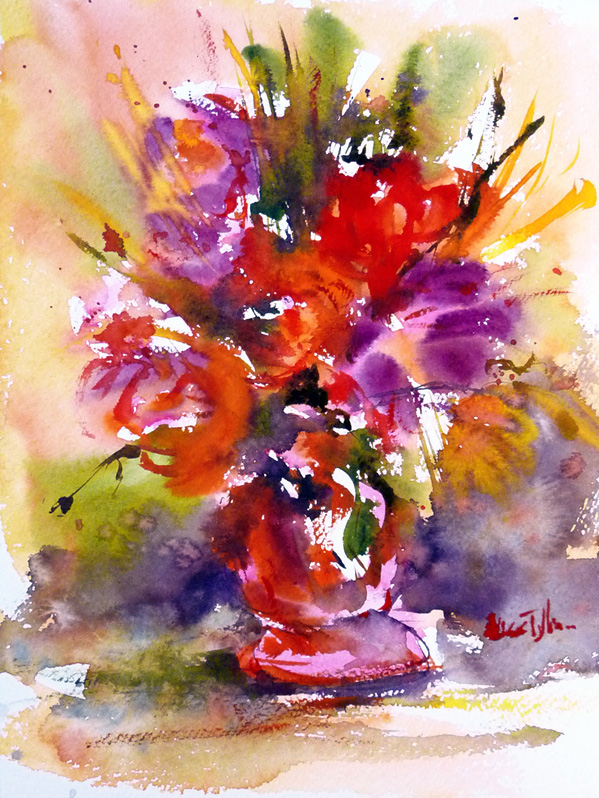
\includegraphics[width=200px, height=200px]{images/bouquet.jpeg}
        \captionof{figure}{Watercolor Bouquet}\footnote{\href{https://i.imgur.com/HA30iGU.jpeg}{https://i.imgur.com/HA30iGU.jpeg}}
    \end{center}
\end{multicols}
\begin{multicols}{2}
    \begin{center}
        \captionsetup{type=figure}
        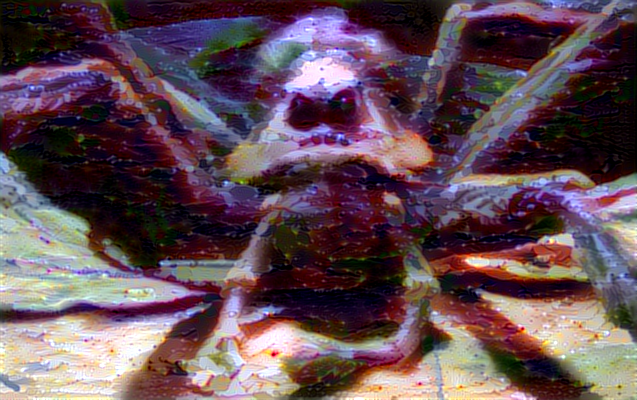
\includegraphics[width=200px, height=200px]{images/comb-aragog-2.png}
        \captionof{figure}{Watercolor Spider (content=0.000000025 style=0.000001)}
    \end{center}
    \begin{center}
        \captionsetup{type=figure}
        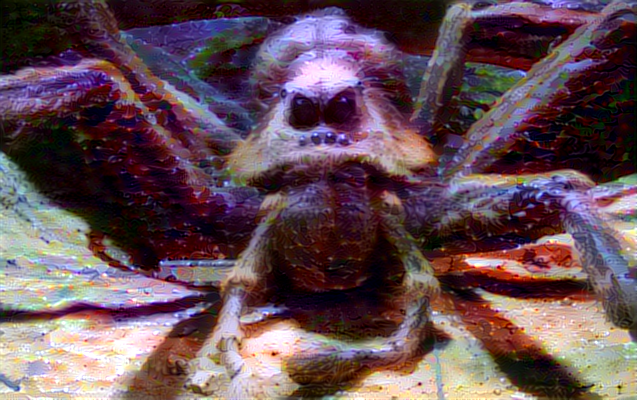
\includegraphics[width=200px, height=200px]{images/comb-aragog-3.png}
        \captionof{figure}{Watercolor Spider (content=0.00001 style=0.000001)}
    \end{center}
\end{multicols}
\clearpage